\documentclass[preprint, 12pt]{aastex}
\usepackage{newtxtext, newtxmath}
\usepackage{graphicx}
\graphicspath{
  {../},
  {/Users/will/Work/RingNebula/WFC3/2013-Geometry/}
}

\newcommand\oiii{[\ion{O}{3}]}
\newcommand\nii{[\ion{N}{2}]}
\newcommand\sii{[\ion{S}{2}]}
\newcommand\ha{\ensuremath{\mathrm{H\alpha}}}
\newcommand\hb{\ensuremath{\mathrm{H\beta}}}
\newcommand\hg{\ensuremath{\mathrm{H\gamma}}}
\newcommand\elec{\ensuremath{_{\mathrm{e}}}}
\newcommand\Te{\ensuremath{T\elec}}
\newcommand\Ne{\ensuremath{n\elec}}
\newcommand\Wav[1]{\ensuremath{\lambda #1}}

\usepackage{geometry}
\geometry{hmargin=0.3cm, vmargin=1.5cm}
\setkeys{Gin}{width=0.6\linewidth, keepaspectratio}  
\usepackage{natbib}
\usepackage{microtype}
\bibliographystyle{apj}
\begin{document}

\newcommand\Pixel{\ensuremath{\Omega_{\mathrm{pix}}}}
\newcommand\Area{\ensuremath{A_{\mathrm{HST}}}}
\newcommand\T[2]{\ensuremath{T_{#1}^{#2}}}
\newcommand\Tlam[1]{\T{\lambda}{#1}}
\newcommand\Tmax[1]{\T{\mathrm{m}}{#1}}
\newcommand\Mean[1]{\ensuremath{\bigl\langle \lambda I_\lambda \bigr\rangle_{#1}}}
\newcommand\MeanC[1]{\ensuremath{\bigl\langle \lambda
    I_\lambda^{\mathrm{cont}} \bigr\rangle_{#1}}}
\newcommand\Color[2]{\ensuremath{k_{#1, #2}}}
\newcommand\COLOR[2]{\ensuremath{\widetilde{k}_{#1, #2}}}
\newcommand\Weff[2]{\ensuremath{\widetilde{W}_{#1, #2}}}
\newcommand\U[1]{\ensuremath{\mathrm{#1}}}
\newcommand\E[1]{\ensuremath{\times 10^{#1}}}
\newcommand\Elam{\ensuremath{\varepsilon_\lambda}}
\newcommand\Constant{\ensuremath{C_{\mathrm{WFC3}}}}
% \newcommand\Narrow{\mathrm{L}}
% \newcommand\Wide{\mathrm{C}}
% \newcommand\Narrow{\mathrm{a}}
% \newcommand\Wide{\mathrm{b}}
\newcommand\Narrow{\mathrm{N}}
\newcommand\Wide{\mathrm{W}}
\newcommand\Contam{\ensuremath{{i'}}} %extra braces are on purpose

\section{Calibration of the WFC3 filters}

In a recent study \citep{ODell:2013b} of NGC~6720, the Ring Nebula,
evidence was found for significant deviations of some WFC3 UVIS
narrow-band filter calibration constants from the pre-launch
determined values given in the WFC3 Instrument Handbook.  Several
observationally important diagnostic line ratios are significantly
impacted by the filter calibrations in question.  It is therefore of
paramount importance to confirm the calibrations under a wider range
of nebular excitation conditions.  The Orion Nebula, M42, provides an
excellent complement to NGC~6720 in this respect, since it is of lower
ionization and temperature, allowing the calibration to be extended to
smaller values of the emission line equivalent widths, where continuum
contamination of the narrow band filters is greater.  At the same
time, extensive high-quality spectrophotometric data exists for this object,
obtained by distinct teams, using multiple telescopes and instruments
(for example, \citealp{Mesa-Delgado:2008b, ODell:2010a}).  This allows
the true spectrum to be determined with a degree of precision and
confidence that is impossible for other objects.

\subsection{Filter count rates}
\label{sec:counts}


Assume we have pipeline-calibrated WFC3 UVIS images, \(R_j\), 
in distinct filters \(j\), 
which are in units \([R_j] = \U{counts\ s^{-1}\ pixel^{-1}}\).  The
effective collecting area of the telescope is \(\Area =
\pi (120\ \U{cm})^2 = 45,239\ \U{cm^2}\) and the solid angle
subtended by each pixel is \(\Pixel = (0.03962'')^2 = 3.6895\E{-14}\
\U{sr}\).  
The transmission profile of the filter is given by
\Tlam{j}, which is the total fractional throughput, 
accounting for camera and detector efficiencies (and including the
fractional area of the primary mirror that is obscured by the secondary).  

A source is observed that has a wavelength-dependent intensity 
\(I_\lambda\) in surface brightness units: 
\([I_\lambda] = \U{erg\ s^{-1}\ cm^{-2}\ sr^{-1}\ \AA^{-1}}\). 
The expected count rate from the source is
\begin{equation}
  \label{eq:rate}
  R_j = \Area\, \Pixel \int_0^\infty \!\!\Elam^{-1} I_\lambda\,
  \Tlam{j} \, d\lambda \quad\quad [R_j] = \U{counts\ s^{-1}\ pixel^{-1}}, 
\end{equation}
where \(\Elam = 10^{8} (h c / \lambda)\) is the photon energy with
\([\Elam] = \U{erg}\) and \([\lambda] = \U{\AA}\). 
If the peak value of the filter transmission profile is \Tmax{j}, then the
``rectangular width'' of the profile is defined as
\begin{equation}
  \label{eq:width}
  W_j = (\Tmax{j})^{-1} \int_0^\infty \!\!\Tlam{j}\, d\lambda 
  \quad\quad [W_j] = \AA.
\end{equation}

For a filter whose pass-band does not contain any strong emission
lines, we can assume that \(I_\lambda\) is a slowly varying function of
\(\lambda\), in which case it is convenient to define an average
intensity over the filter passband:
\begin{equation}
  \label{eq:average}
  \Mean{j} = \int_0^\infty \!\!\lambda I_\lambda \Tlam{j} \, d\lambda \,
  \Bigg/\! \int_0^\infty \!\!\Tlam{j} \, d\lambda .
\end{equation}
Hence, from equations~(\ref{eq:rate}--\ref{eq:average}) we may write
the count rate in this case as
\begin{equation}
  \label{eq:continuum}
  R_j = \Constant\, \Mean{j}\, \Tmax{j}\, W_j , 
\end{equation}
where \(\Constant = 10^{-8} \Area\, \Pixel / (h c) = 0.0840241\ \U{counts\
  cm^2\
  sr\ erg^{-1}\ \AA^{-1}\ pixel^{-1}}\). 

Next, consider a filter whose pass-band contains 
one or more narrow emission lines \(i\), 
each with central wavelength \(\lambda_i\) 
and wavelength-integrated intensity \(I_i\),
plus a smoothly varying continuum \(I_\lambda^{\mathrm{cont}}\):
\begin{equation}
  \label{eq:line-plus-cont}
  I_\lambda = I_\lambda^{\mathrm{cont}} + 
  \sum_{i=1, n} I_i\, \delta(\lambda - \lambda_i)  ,
\end{equation}
where \(\delta\) denotes the Dirac delta function.
The equivalent width, or EW, of each line is
\(-E_i\) with respect to its local continuum, where
\begin{equation}
  \label{eq:EW}
  E_i = I_i / I_\lambda^i \quad\quad [E_i] = \U{\AA}, 
\end{equation}
and in which \(I_\lambda^i \equiv I_\lambda^{\mathrm{cont}} (\lambda \!=\!
\lambda_i)\) is the continuum intensity at the line wavelength.  
The filter transmission at the line wavelength is denoted 
\(\T{i}{j} \equiv \Tlam{j}(\lambda\!=\!\lambda_i)\)
and the color term \(\Color{j}{i}\) is defined as 
the ratio of the mean continuum intensity in the filter to the
continuum intensity at the line wavelength:
\begin{equation}
  \label{eq:line-color}
  \Color{j}{i} \equiv \frac{\MeanC{j}}{\lambda_i I_\lambda^i} . 
\end{equation}
Note that \(\Color{j}{i}\) will be very close to unity so long as the
filter is narrow.  
It is also convenient to define an ``effective width'' of the filter 
with respect to the emission line: 
\begin{equation}
  \label{eq:effective}
  \Weff{j}{i} \equiv \Color{j}{i} \frac{\Tmax{j}}{\T{i}{j}} W_j .
\end{equation}
From the foregoing, the count rate in this case is found to be
\begin{equation}
  \label{eq:R-line-plus-cont}
  R_j 
  % = \Constant\, \MeanC{j} 
  % \left(
  %    \Tmax{j} W_j + \T{i}{j} E_i / \Color{j}{i}
  % \right) 
  = \Constant\, \MeanC{j} \, \Tmax{j} W_j 
  \left(
     1 + \sum_{i=1,n} E_i / \Weff{j}{i}
  \right) 
  .
\end{equation}

\newcommand\multicorrel[2]{
    \includegraphics[width=0.33\linewidth]{ring-#1-absolute}%
    \includegraphics[width=0.33\linewidth]{odh-#1-absolute}%
    \includegraphics[width=0.33\linewidth]{adal-#1-absolute}%
}

\begin{figure}[p]
  \centering
  \multicorrel{F547M}{green}
  \caption{Full-filter observed versus synthetic count rates for F547M}
  \label{fig:multicorrel-continuum}
\end{figure}

\begin{figure}[p]
  \centering
  \multicorrel{F658N}{red}\\
  \multicorrel{F656N}{red}\\
  \multicorrel{F673N}{red}
  \caption{Full-filter observed versus synthetic count rates for red lines}
  \label{fig:multicorrel-red}
\end{figure}

\begin{figure}[p]
  \centering
  \multicorrel{F502N}{green}\\
  \multicorrel{F487N}{green}\\
  \multicorrel{F469N}{green}
  \caption{Full-filter observed versus synthetic count rates for green lines}
  \label{fig:multicorrel-green}
\end{figure}

\begin{figure}[p]
  \centering
  \multicorrel{FQ575N}{red}\\
  \multicorrel{FQ672N}{red}\\
  \multicorrel{FQ674N}{red}\\
  \caption{Full-filter observed versus synthetic count rates for red quad lines}
  \label{fig:multicorrel-red-quad}
\end{figure}
\begin{figure}[p]
  \centering
  \multicorrel{FQ437N}{blue}\\
  \multicorrel{FQ436N}{blue}\\
  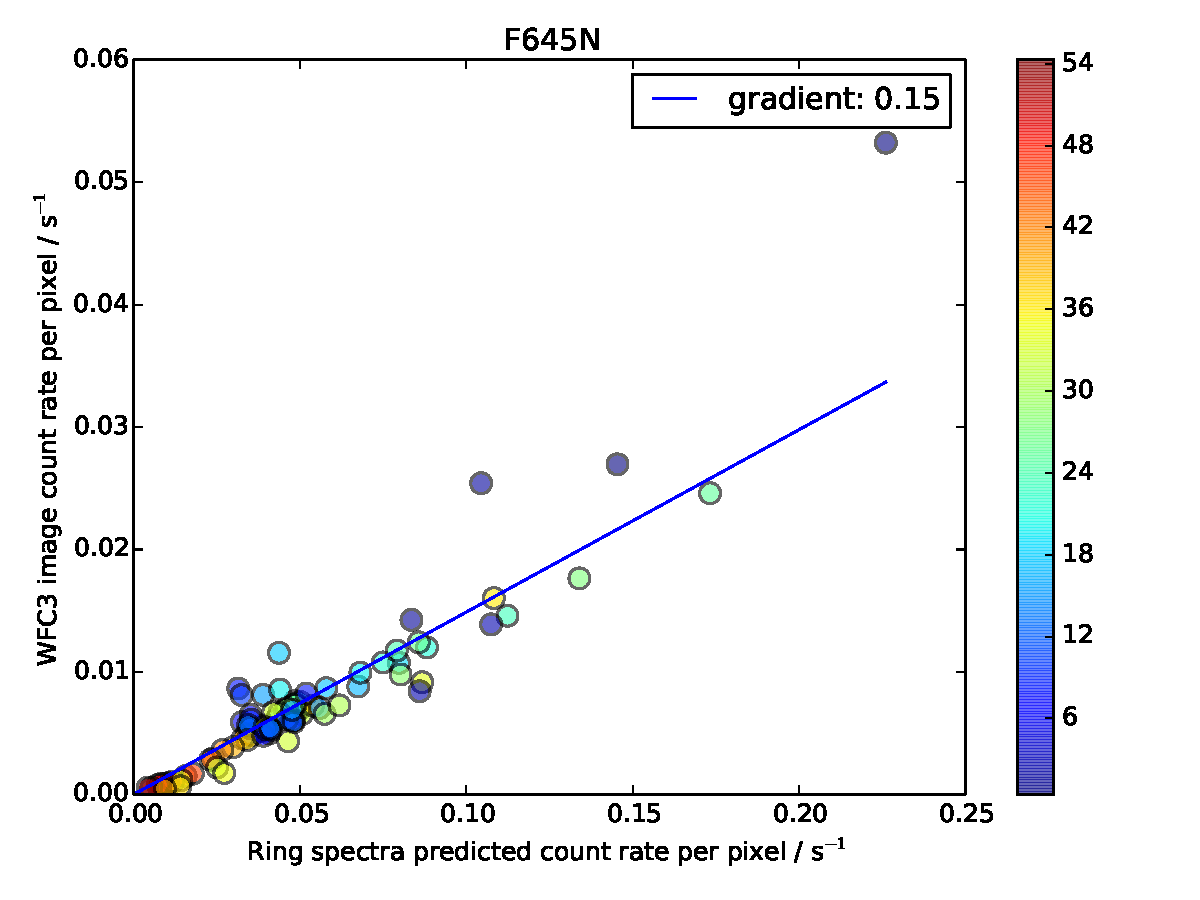
\includegraphics[width=0.33\linewidth]{ring-F645N-absolute}%
  \caption{Full-filter observed versus synthetic count rates for blued quad lines}
  \label{fig:multicorrel-blue-quad}
\end{figure}

\subsection{Filter Ratio Type I}
\label{sec:typeI}

We first consider finding the ratio between the count rate in a
narrow filter (\(j = \Narrow\)) that contains a single emission line, 
given by equation~(\ref{eq:R-line-plus-cont}) with \(n=1\), 
and the rate in a broader filter (\(j = \Wide\)) that passes only
continuum, given by equation~(\ref{eq:continuum}). 
It is convenient to define a filter-to-filter continuum color: 
\begin{equation}
  \label{eq:cont-color}
  \Color{\Narrow}{\Wide} \equiv \frac{\MeanC{\Narrow}}{\MeanC{\Wide}} ,
\end{equation}
such that the ratio is given by
\begin{equation}
  \label{eq:ratio-type-I}
  \frac{R_\Narrow}{R_\Wide} = 
  \Color{\Narrow}{\Wide} \frac{\Tmax{\Narrow} W_\Narrow}{\Tmax{\Wide} W_\Wide}
  \left(
    1 + \frac{E_i}{\Weff{\Narrow}{i}}
  \right) .
\end{equation}
Note that the factor \(E_i / \Weff{\Narrow}{i}\) gives the relative
importance of the line over the continuum in the narrow filter, and
that the filter count ratio is a linear function of the line
equivalent width. 

\subsection{Filter Ratio Type IIa}
\label{sec:typeIIa}
If the \emph{same} emission line is present in the pass band of the
wide filter as well as the narrow filter, then it is necessary to use
equation~(\ref{eq:R-line-plus-cont}) for both filters.  
However, in this case one commonly has \(E_i \ll \Weff{\Wide}{i}\) and so
it is sufficient to expand the ratio in powers of \(E_i /
\Weff{\Wide}{i}\):
\begin{equation}
  \label{eq:ratio-type-II}
    \frac{R_\Narrow}{R_\Wide} = 
  \Color{\Narrow}{\Wide} \frac{\Tmax{\Narrow} W_\Narrow}{\Tmax{\Wide} W_\Wide}
  \left(
    1 + \frac{E_i}{\Weff{\Narrow}{i}}
  \right) 
  \left(
    1 - \frac{E_i}{\Weff{\Wide}{i}}
  \right)
  + \mathcal{O}\left[ 
    \left(\frac{E_i}{\Weff{\Wide}{i}}\right)^2
  \right]
  .
\end{equation}
If only the term linear in \(E_i / \Weff{\Wide}{i}\) is retained, the
ratio becomes
\begin{equation}
  \label{eq:ratio-type-II-approx}
    \frac{R_\Narrow}{R_\Wide} \simeq
  \Color{\Narrow}{\Wide} \frac{\Tmax{\Narrow} W_\Narrow}{\Tmax{\Wide} W_\Wide}
  \left(
    1 + E_i \left( \frac{1}{\Weff{\Narrow}{i}} - \frac{1}{\Weff{\Wide}{i}} \right)
    - \frac{E_i^2}{\Weff{\Narrow}{i} \Weff{\Wide}{i}}
  \right) 
  .
\end{equation}
Thus the effect of a small ``contamination'' of the wide filter by the
emission line is to reduce the slope of the relation between line
equivalent width and filter ratio, and also to introduce a slight
negative curvature for the highest equivalent widths.

\subsection{Filter Ratio Type IIb}
\label{sec:typeIIb}
If the wide filter is contaminated by one or more \emph{different} lines,
\Contam{}, then similar considerations apply.
But in this case, the shape of the
EW--filter ratio relation is unaffected and the contamination is best
accommodated by simply modifying the filter-to-filter color ratio to
include the contribution of the contaminating lines:
\begin{equation}
  \label{eq:color-correct-IIb}
  \COLOR{\Narrow}{\Wide} \equiv \frac{\MeanC{\Narrow}}{\Mean{\Wide}}
  = \Color{\Narrow}{\Wide} 
  \left( 1 + \sum_{\Contam \ne i}\frac{E_\Contam}{\Weff{\Wide}{\Contam}} \right)^{-1}
  .
\end{equation}
The ratio then retains the same simple form as for Type~I: 
\begin{equation}
  \label{eq:ratio-type-IIb}
  \frac{R_\Narrow}{R_\Wide} = 
  \COLOR{\Narrow}{\Wide} \frac{\Tmax{\Narrow} W_\Narrow}{\Tmax{\Wide} W_\Wide}
  \left(
    1 + \frac{E_i}{\Weff{\Narrow}{i}}
  \right) .
\end{equation}
Note that no series expansion has been made in this case, and the
above expressions are formally valid for arbitrarily high \(\sum E_\Contam
/ \Weff{\Wide}{\Contam}\).  However, if \(E_\Contam >
\Weff{\Wide}{\Contam}\) for any particular line, 
then the variations in \(R_\Narrow / R_\Wide\)
may be driven by variations in \(E_\Contam\) as much as by variations
in \(E_i\), in which case the apparent simplicity of
equation~(\ref{eq:ratio-type-IIb}) is illusory. 

\subsection{Filter Ratio Type III}
\label{sec:typeIII}

Two lines in the same filter -- \textit{TODO}

\subsection{Relative calibration within filter sets}
\label{sec:application}

In the following, all 3-figure IDs denote a particular filter,~\(j\). 
For example \(W_{547}\) for the rectangular width of filter
F547M.  
On the other hand, all 4-figure IDs denote a particular emission line,~\(i\). 
For example \(E_{6583}\) for the equivalent width of \nii{}
\Wav{6583}.

\subsubsection{F658N, FQ575N, and F547M: \nii{} nebular and auroral lines}
\label{sec:658-575-547}

The narrow-band filter F658N (\(W_{658} \simeq 28~\U{\AA}\)) passes
the strong nebular line \nii{} \Wav{6583}, which has an equivalent
width of \(E_{6583} = 200\textrm{--}400~\U{\AA}\) in M42, rising to
more than 3000~\U{\AA} in the the main ring of NGC~6720.
The continuum contribution to the filter is therefore always small, of
order 10\% in M42 and \(< 1\%\) in NGC~6720.

The even narrower quad filter FQ575N (\(W_{575} \simeq 21~\U{\AA}\))
passes the relatively weak auroral line \nii{} \Wav{5755}, which has
an equivalent width of \(E_{5755} = 2\textrm{--}10~\U{\AA}\) in M42,
reaching values as high as \(100~\U{\AA}\) in NGC~6720.  We therefore
expect a significant continuum contribution to the filter of 50--90\%
in M42 and \(\sim 20\%\) in NGC~6720.

The medium-band filter F547M (\(W_{547} \simeq 650~\U{\AA}\)) is
dominated by continuum emission in lower excitation sources such as
M42, where the total EW of emission lines in the filter is generally
\(< 20~\U{\AA}\), corresponding to a few percent of the filter flux.
In NGC~6720 on the other hand, \nii{} \Wav{5755} and other lines such
as [\ion{N}{1}] \Wav{5198,5200} and \ion{He}{2} \Wav{5411} can sum to
a total EW of 100--300~\AA{} and contribute 15--30\% of the total
F547M flux.

The ratio \(R_{658} / R_{547}\) is therefore of Type~IIa, so that if
\(E_{6583}\) and \(\COLOR{658}{547}\) can be measured independently
from spectrophotometry for a sufficently large range of \(E_{6583}\),
for which co-spatial WFC3 observations are available, then the filter constants can be determined graphically from the slope and
intercept of the EW--ratio relation as follows:
\begin{equation}
  \label{eq:658-547}
  \frac{R_{658}}{\COLOR{658}{547} R_{547}} = 
  r_0 \bigl( 
  1 + q_1 E_{6583}  
  \bigr) , 
\end{equation}
where
\[
r_0 = \frac{\Tmax{658} W_{658}}{\Tmax{547} W_{547}} ;
\quad\quad
q_1 = \frac{1}{\Weff{658}{6583}} .
\]

The ratio \(R_{575} / R_{547}\) is of Type~IIab and should obey a relation:
\begin{equation}
  \label{eq:575-547}
  \frac{R_{575}}{\COLOR{575}{547} R_{547}} = 
  r_0 \biggl( 
    1 + q_1 E_{5755} \bigl( 
      1 - q_2 E_{5755}
    \bigr)
  \biggr)
\end{equation}
where
\[
r_0 = \frac{\Tmax{575} W_{575}}{\Tmax{547} W_{547}} ;
\quad\quad
q_1 = \frac{\Weff{547}{5755} - \Weff{575}{5755}}{\Weff{547}{5755} \, \Weff{575}{5755}} ;
\quad\quad
q_2 = \frac{1}{\Weff{547}{5755} - \Weff{575}{5755}} .
\]

\begin{figure}
  \centering
  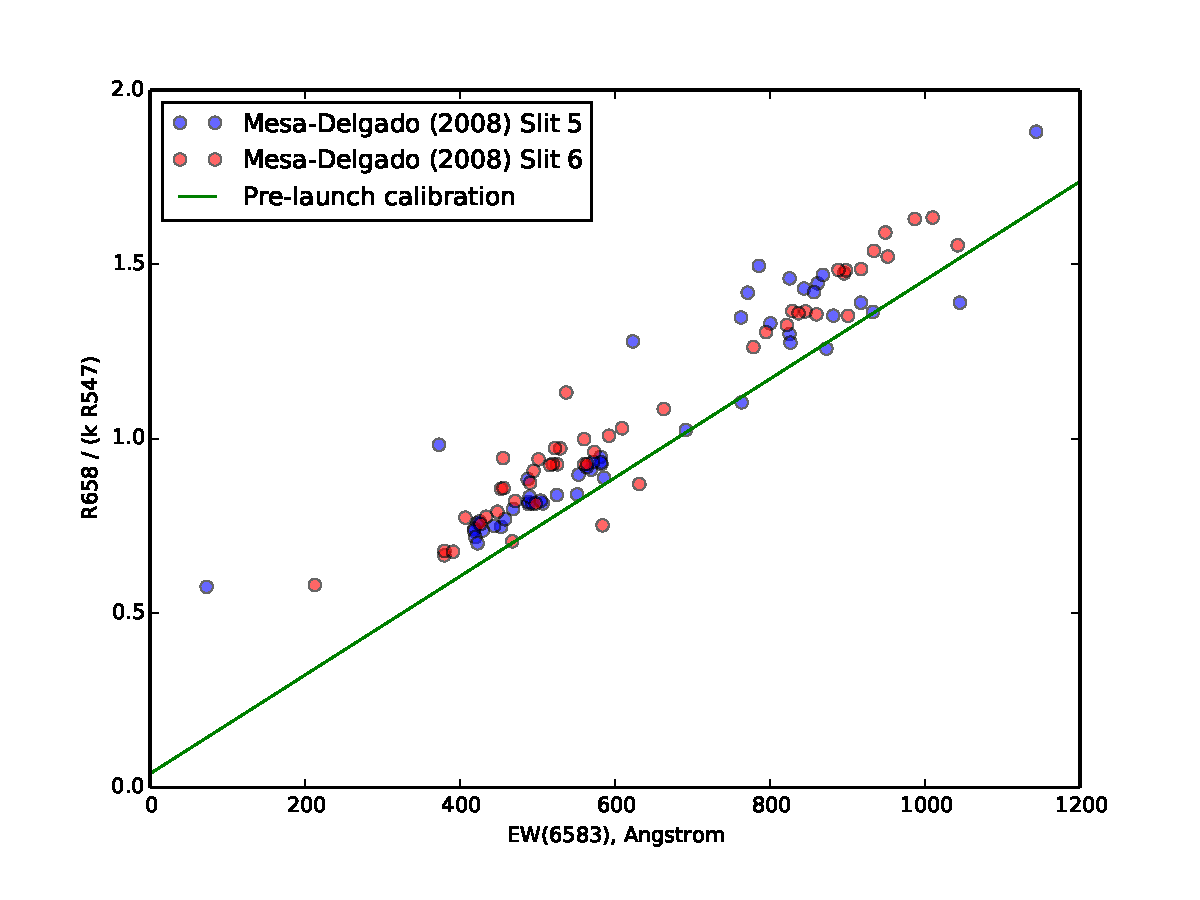
\includegraphics[width=0.8\linewidth]{adal-w6583-calibration}
  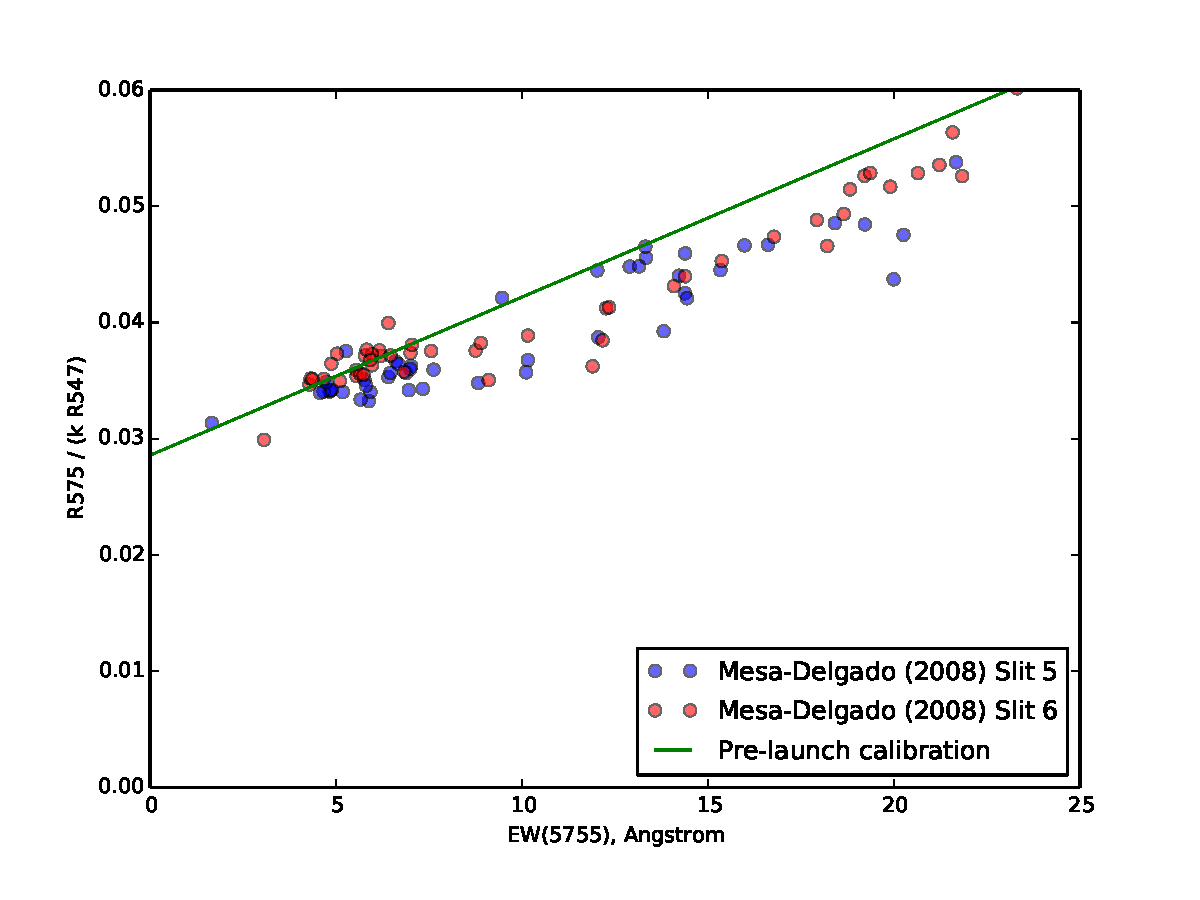
\includegraphics[width=0.8\linewidth]{adal-w5755-calibration}
  \caption{Preliminary calibration of 5755 and 6583}
  \label{fig:adal}
\end{figure}

\subsubsection{F673N, FQ672N, and FQ674N: \sii{} nebular doublet}
\label{sec:673-672-674}

\subsubsection{FQ436N, FQ437N, F502N, and F547M: H\(\gamma\) and
  \oiii{} nebular and auroral lines}
\label{sec:437}
This is going to be the most challenging. 


\subsection{Absolute calibration}
\label{sec:absolute}

\newcommand\LineID[1]{\multicolumn{1}{c}{#1}}
\begin{figure}
  \centering
  \begin{tabular}{ll}
    (a) & (b) \\
    \LineID{F656N: \ha{} \Wav{6563}}& \LineID{F486N: \hb{} \Wav{4861}} \\
    \includegraphics[width=0.48\linewidth]{ring-F656N-F547M-6563-comparison} &
    \includegraphics[width=0.48\linewidth]{ring-F487N-F547M-4861-comparison}
    \\
    (c) & (d) \\
    \LineID{F658N: \nii{} \Wav{6583}}& \LineID{F502N: \oiii{} \Wav{5007}} \\
    \includegraphics[width=0.48\linewidth]{ring-F658N-F547M-6583-comparison} &
    \includegraphics[width=0.48\linewidth]{ring-F502N-F547M-5007-comparison}
  \end{tabular}

  \caption{Strong lines versus continuum.  Ring Nebula calibration.
    All are consistent with the pre-launch calibration.}
  \label{fig:strong}
\end{figure}


\begin{figure}
  \centering
  \begin{tabular}{ll}
    (a) & (b) \\
    \LineID{F673N: \sii{} \Wav{6716+31}}& 
    \LineID{F469N: \ion{He}{2} \Wav{4686}} \\
    \includegraphics[width=0.48\linewidth]{ring-F673N-F547M-6716-comparison} &
    \includegraphics[width=0.48\linewidth]{ring-F469N-F547M-4686-comparison}
    \\
    (c) & (d) \\
    \LineID{FQ672N: \sii{} \Wav{6716}}& \LineID{FQ674N: \sii{} \Wav{6731}} \\
    \includegraphics[width=0.48\linewidth]{ring-FQ672N-F547M-6716-comparison} &
    \includegraphics[width=0.48\linewidth]{ring-FQ674N-F547M-6731-comparison}
  \end{tabular}

  \caption{Medium lines versus continuum.  Ring Nebula
    calibration. (a)~Broad \sii{} nebular filter. \emph{Note that I need to
      include the EW of both lines in the x-axis.} (b)~\ion{He}{2}
    filter.  \emph{I still need to correct for the [\ion{Ar}{4}] and
      \ion{He}{1} but that should only be a 10\% effect}. (c) and
    (d)~Narrow \sii{} nebular filters.  There is a significant
    deviation from the pre-launch calibration for FQ674N.}
  \label{fig:strong}
\end{figure}


\begin{figure}
  \centering
  \begin{tabular}{ll}
    (a) & (b) \\
    \LineID{FQ575N: \nii{} \Wav{5755}}& 
    \LineID{FQ437N: \oiii{} \Wav{4363}} \\
    \includegraphics[width=0.48\linewidth]{ring-FQ575N-F547M-5755-comparison} &
    \includegraphics[width=0.48\linewidth]{ring-FQ437N-F547M-4363-comparison}
    \\
    (c) & (d) \\
    \LineID{FQ436N: \hg{} \Wav{4340}}&  \\
    \includegraphics[width=0.48\linewidth]{ring-FQ436N-F547M-4340-comparison} &
    
  \end{tabular}

  \caption{Weak lines versus continuum.  Ring Nebula calibration.}
  \label{fig:strong}
\end{figure}


\section{Raw filter comparison}
\label{sec:raw}

\newcommand\orioncomparison[2]{
  %% arg 1: Filter (e.g., F547M)
  %% arg 2: Band (e.g., red)
  \begin{figure}[p]
    \centering
    \includegraphics[width=\linewidth]{manu-#1-#2-maps}\\
    \includegraphics[width=0.33\linewidth]{odh-#1-absolute}%
    \includegraphics[width=0.33\linewidth]{manu-#1-#2-absolute}%
    \includegraphics[width=0.33\linewidth]{adal-#1-absolute}%
    \caption{Orion Nebula raw filter comparison for #1}
    \label{fig:orioncomparison-#1-#2}
  \end{figure}
}

\newcommand\ringcomparison[1]{
  %% arg: Filter, e.g., FQ575N
  \begin{figure}[p]
    \centering
    \includegraphics[width=0.33\linewidth]{ring-#1-absolute}%
    \includegraphics[width=0.33\linewidth]{ring-profile-pa60-#1}%
    \includegraphics[width=0.33\linewidth]{ring-profile-pa150-#1}%
    \caption{Ring Nebula raw filter comparison for #1}
    \label{fig:ringcomparison-#1}
  \end{figure}
}

\newcommand\multicomparison[2]{
  \orioncomparison{#1}{#2}
  \ringcomparison{#1}\clearpage
}


\multicomparison{F658N}{red}
\multicomparison{F656N}{red}
\multicomparison{F673N}{red}
\multicomparison{F502N}{green}
\multicomparison{F487N}{green}
\multicomparison{F469N}{green}

\multicomparison{F547M}{green}

\multicomparison{FQ575N}{red}
\multicomparison{FQ672N}{red}
\multicomparison{FQ674N}{red}
\multicomparison{FQ437N}{blue}
\multicomparison{FQ436N}{blue}

\ringcomparison{F645N}


\bibliography{BibdeskLibrary-slavoj}

\end{document}
